\documentclass[25pt, a0paper, portrait, blockverticalspace=.5cm]{tikzposter}
\usepackage[utf8]{inputenc}
\usepackage{amssymb,amsfonts,amsmath,mathtext,mathtools}
\usepackage{xfrac}
\usepackage{enumitem}

\usepackage{makecell}
\usepackage{amsmath}

\let\vec\oldvec
\newcommand{\vec}[1]{\boldsymbol{#1}}

\title{\parbox{\linewidth}
	{\centering
		Transition energy crossing in harmonic RF at proton synchrotron U-70
\\		
}}

\author{S. Kolokolchikov\textsuperscript{1,2}*, Y. Senichev\textsuperscript{1,2}, V. Kalinin\textsuperscript{3}}
\institute{
	\textsuperscript{1} Institute for Nuclear Research of the Russian Academy of Sciences, Moscow, Russia\\
	\textsuperscript{2} Moscow Institute of Physics and Technology, Dolgoprudny, Russia\\
	\textsuperscript{3} Institute for High Energy Physics, Protvino, Russia\\
	*sergey.bell13@gmail.com
}
\usetheme{Simple}
\usecolorstyle{Russia}
\colorlet{blocktitlefgcolor}{black}

\usepackage{caption}
\captionsetup{font=large}
\usepackage{multicol}
\setlength\columnsep{1.5cm}

\begin{document}

\maketitle

\begin{columns}
\column{.33}

\block{INTRODUCTION}{

\par This work is devoted to the study of the transition energy crossing in harmonic RF. For this purpose, the paper presents longitudinal motion modelling, including high order of momentum compaction factor, various impedances and intensities. Experimental data of a session on the synchrotron U-70, where the crossing of transition energy is carried out by the method of rapid change of transition energy in harmonic RF. Also considered crossing without an additional jump.
}

\column{.33}
\block{Longitudinal motion}{

\par General longitudinal equations of motion for one harmonic RF [1]

\begin{equation}
\left\{\begin{array}{c}
\frac{d \tau}{d t}=-\frac{\eta}{\beta^2 E_0} \Delta E \\
\frac{d \Delta E}{d t}=\frac{Z e}{A} \frac{\omega_0}{2 \pi} V\left[\sin \left(\phi_s-h \omega_0 \tau\right)-\sin \phi_s\right]
\end{array}\right.
\end{equation}
\par where $\tau$ -- deviation the reference, $\beta c$ -- speed, $\omega_0=\sfrac{2\pi}{T_0}$ -- angular frequency and corresponding time, $h$ -- harmonic time, $V$ -- RF amplitude, $\phi_s$ -- phase of reference particle, slip-factor $\eta\left(\delta\right)=-\left(\eta_0+\eta_1\delta+\cdots\right)$. 

}
\column{.33}
\block{Impedance influence}{
\par Impedance is a function that combine all electro-magnetic effects that influence on beam.

\begin{equation}
[\mathbf{E}+\mathbf{v} \times \mathbf{B}(t, \theta)]_{\|}=-\frac{1}{2 \pi R_0} Z_{\|}(\omega) J_{\|}(t, \theta)
\end{equation}

In simple cases, space charge impedance is a negative pure inductive, here will consider $(Z_{\|}/n)_{SC}=-10i$. But ring contains different elements that can lead to positive inductance $(Z_{\|}/n)_{U-70}=+10i$.[2]
}
\end{columns}

\begin{columns}
\column{.5}
\block{Transition crossing}{

\par The synchrotron tune depend on $\eta$. Thus, near transition $\eta \rightarrow 0$ the motion become \textbf{non-adiabatic}. Moreover, $\eta$ depend on $\delta$ and high-orders lead to \textbf{non-linearity}. [3]

		\begin{minipage}{0.5\linewidth}
		\begin{equation}
		\tau_{\mathrm{ad}}=\left(\frac{\pi \beta^2 m c^2 \gamma_{t r}^4}{\dot{\gamma} \omega_0^2 h e V\left|\cos \phi_{\mathrm{s}}			\right|}\right)^{1 / 3}
		\end{equation}
		\end{minipage}
		\begin{minipage}{0.5\linewidth}
		\begin{equation}
		\tau_{n l}=\frac{\eta_1 \hat{\delta}}{2 \dot{\gamma} / \gamma_{t r}{ }^3}=\gamma_{t r} \frac{3 / 2 \beta^2+\gamma_{t r}^2 			\alpha_1}{2 \dot{\gamma}}\hat{\delta}
		\end{equation}
		\end{minipage}

		\begin{minipage}{0.5\linewidth}
			\begin{tikzpicture}
			\node (cone) at (0,0) {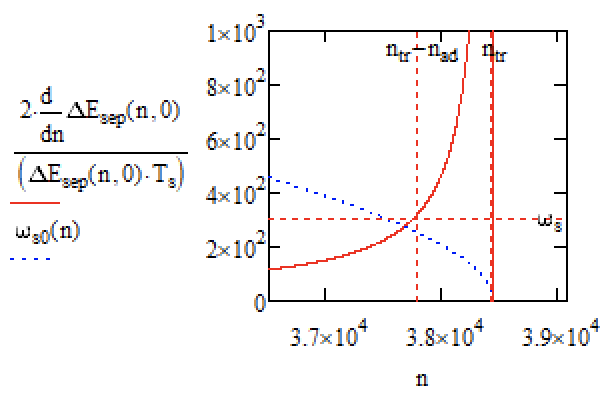
\includegraphics[width=\linewidth]{TEXPaper/img/adiabat2}};
			\end{tikzpicture}
		\end{minipage}
		\begin{minipage}{0.5\linewidth}
			\begin{tikzpicture}
			\node (cone) at (0,0) {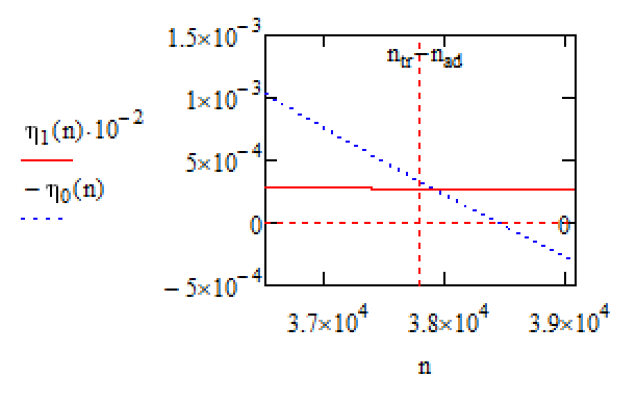
\includegraphics[width=\linewidth]{TEXPaper/img/nonlin}};
			\end{tikzpicture}
		\end{minipage}


\par Considered transition energy crossing. Then $\eta$ change sign, the synchrotron phase also change as $2\phi_{s}$. Represents two solver variants using for modeling, 'simple' and 'exact'. Also 'exact' solution for high-orders of momentum compaction factor. [4]

		\begin{minipage}{0.33\linewidth}
			\begin{tikzpicture}
			\node (cone) at (0,0) {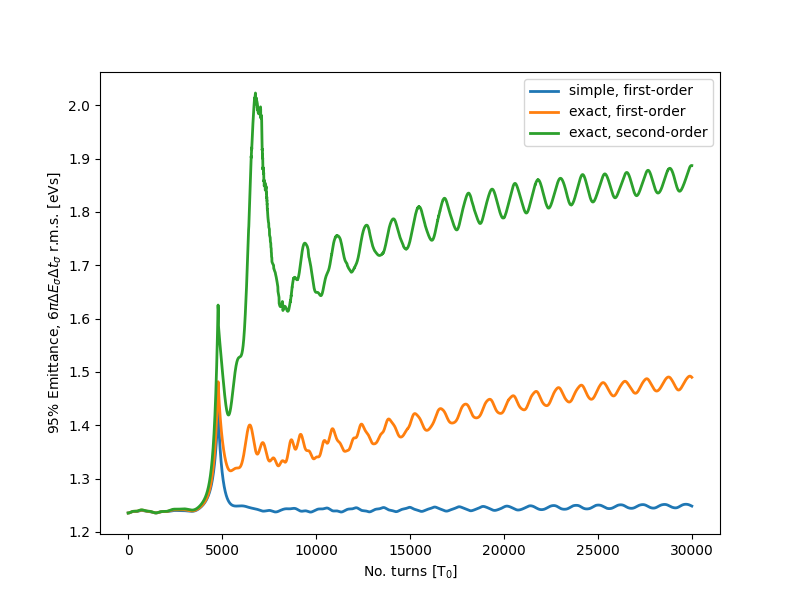
\includegraphics[width=\linewidth]{TEXPaper/img/several_bunch_emittance_wo_jump}};
			\end{tikzpicture}
		\end{minipage}
		\begin{minipage}{0.33\linewidth}
			\begin{tikzpicture}
			\node (cone) at (0,0) {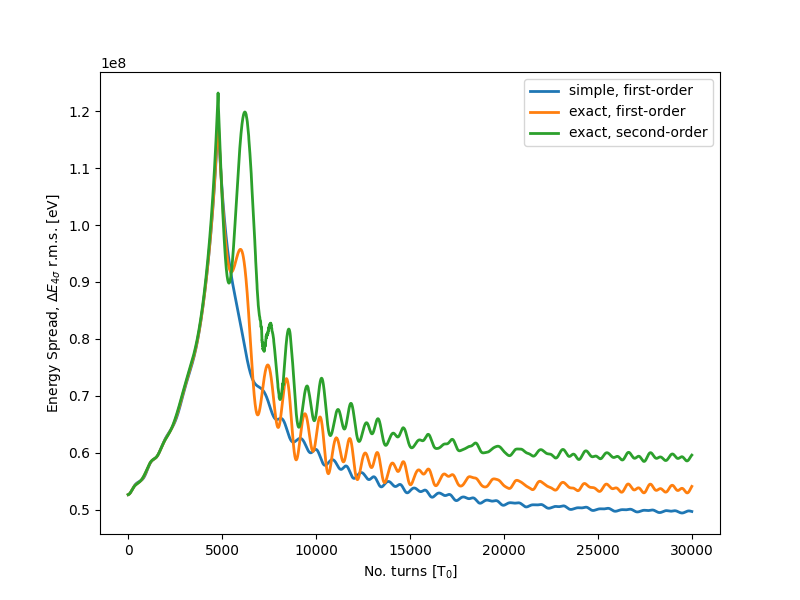
\includegraphics[width=\linewidth]{TEXPaper/img/several_bunch_energy_spread_wo_jump}};
			\end{tikzpicture}
		\end{minipage}
		\begin{minipage}{0.33\linewidth}
			\begin{tikzpicture}
			\node (cone) at (0,0) {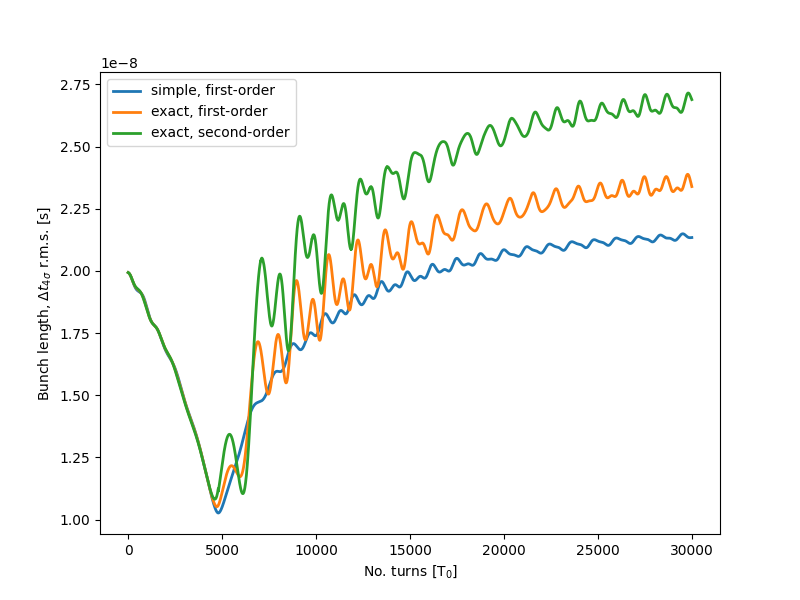
\includegraphics[width=\linewidth]{TEXPaper/img/several_bunch_length_evol_wo_jump}};
			\end{tikzpicture}
		\end{minipage}

\par Pure inductive impedances used $Z_{\|}/n=\pm10i$ for various intensities.

		\begin{minipage}{0.33\linewidth}
			\begin{tikzpicture}
			\node (cone) at (0,0) {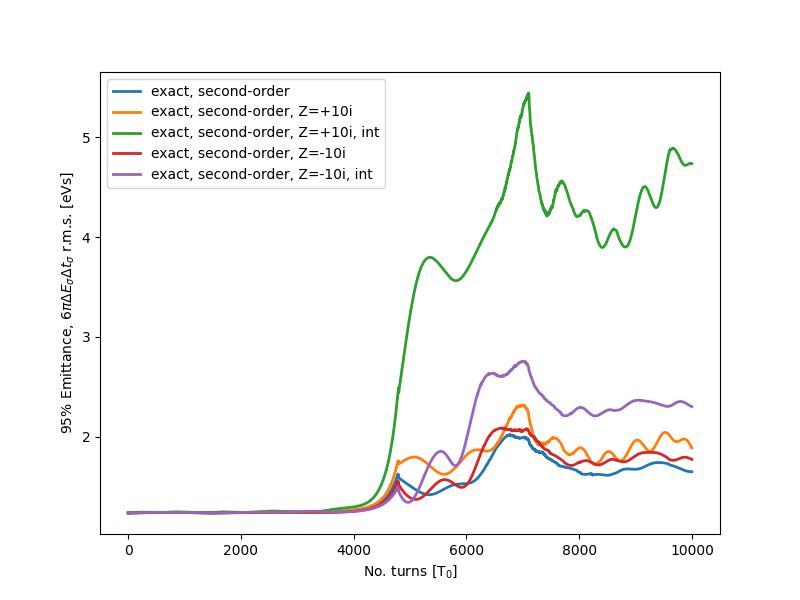
\includegraphics[width=\linewidth]{TEXPaper/img/several_bunch_emittance_wo_jump_sc}};
			\end{tikzpicture}
		\end{minipage}
		\begin{minipage}{0.33\linewidth}
			\begin{tikzpicture}
			\node (cone) at (0,0) {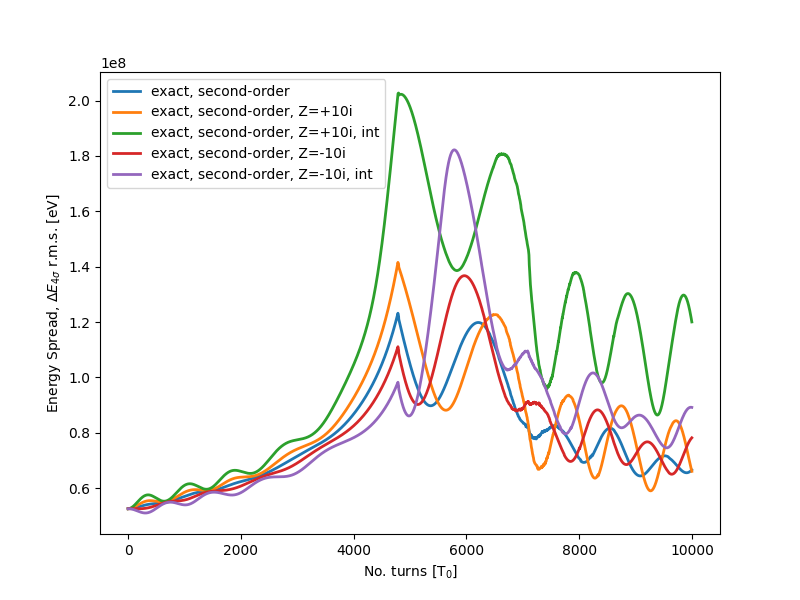
\includegraphics[width=\linewidth]{TEXPaper/img/several_bunch_energy_spread_wo_jump_sc}};
			\end{tikzpicture}
		\end{minipage}
		\begin{minipage}{0.33\linewidth}
			\begin{tikzpicture}
			\node (cone) at (0,0) {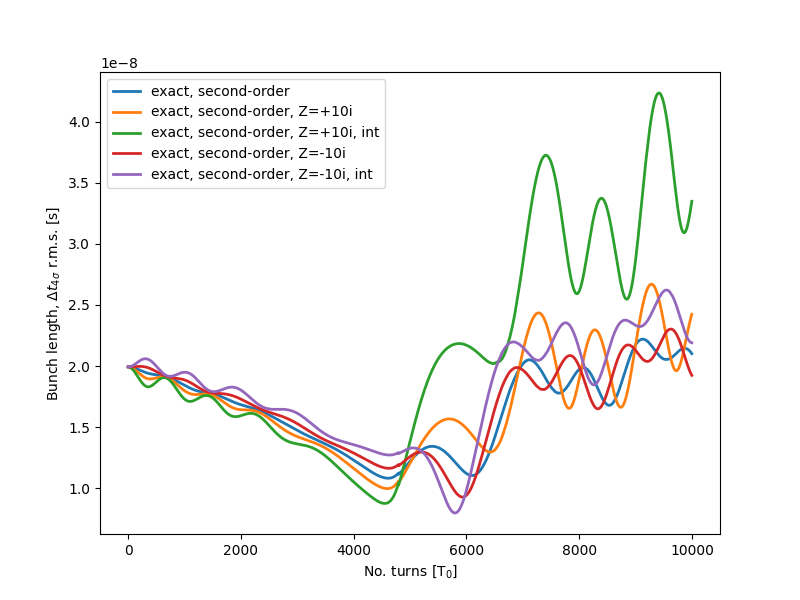
\includegraphics[width=\linewidth]{TEXPaper/img/several_bunch_length_evol_wo_jump_sc}};
			\end{tikzpicture}
		\end{minipage}
\par Emittance growth is observed, especially for high intensity beams.
}
		
\block{Dispersion modulation}{
		
		\begin{minipage}{0.33\linewidth}
			\par In general, momentum compaction factor can be calculated as an integral
			\begin{equation}
				\alpha=\frac{1}{C} \int_0^{\mathrm{C}} \frac{D(s)}{\rho(s)} d s
			\end{equation}
		\end{minipage}
		\begin{minipage}{0.33\linewidth}
			\begin{tikzpicture}
			\node (cone) at (0,0) {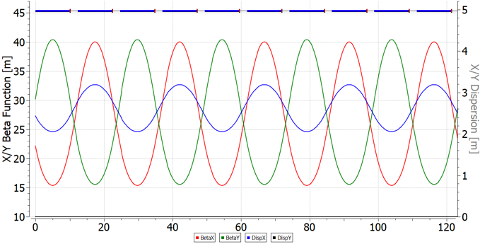
\includegraphics[width=\linewidth]{TEXPaper/img/twiss_1}};
			\end{tikzpicture}
		\end{minipage}
		\begin{minipage}{0.33\linewidth}
			\begin{tikzpicture}
			\node (cone) at (0,0) {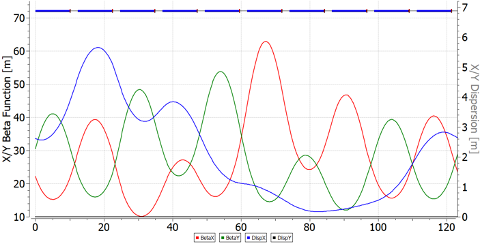
\includegraphics[width=\linewidth]{TEXPaper/img/twiss_2}};
			\end{tikzpicture}
		\end{minipage}
		\par Modulation is carried out by quadrupoles in blocks 2 and 8. And located at half a period ${\Delta\nu}_{x,y}=0.5\times0.5$ and have opposite polarities. [2, 5]
		
}		
\column{.5}
\block{$\gamma$-transition jump}{
	
		\begin{minipage}{0.2\linewidth}
			\par Principal scheme of first order of momentum compaction factor $\alpha$ over turns. And $\eta_{0}$, what defines the longitudinal motion.
		\end{minipage}
		\begin{minipage}{0.4\linewidth}
			\begin{tikzpicture}
			\node (cone) at (0,0) {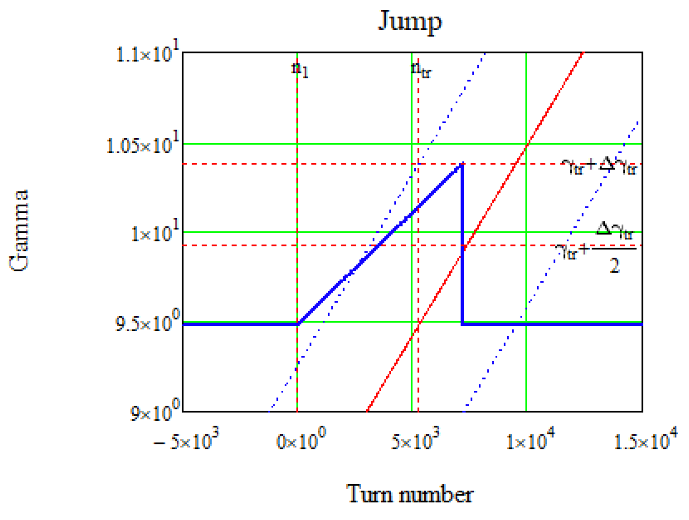
\includegraphics[width=\linewidth]{TEXPaper/img/alpha_jump}};
			\end{tikzpicture}
		\end{minipage}
		\begin{minipage}{0.4\linewidth}
			\begin{tikzpicture}
			\node (cone) at (0,0) {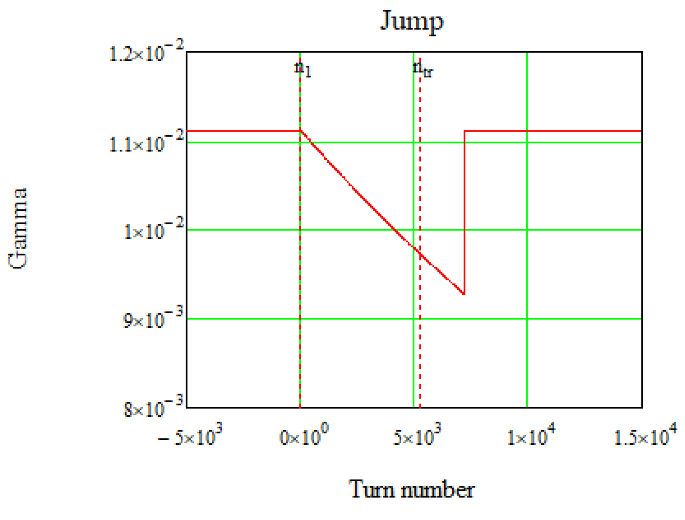
\includegraphics[width=\linewidth]{TEXPaper/img/eta_jump}};
			\end{tikzpicture}
		\end{minipage}

\par Jump is applied for longitudinal motion. And seems identically for various cases.
		
		\begin{minipage}{0.33\linewidth}
			\begin{tikzpicture}
			\node (cone) at (0,0) {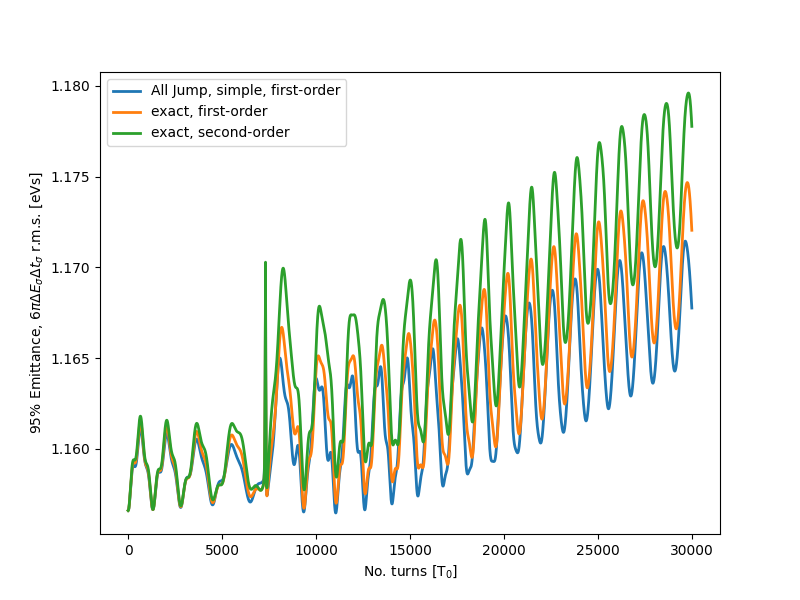
\includegraphics[width=\linewidth]{TEXPaper/img/jump_several_bunch_emittance}};
			\end{tikzpicture}
		\end{minipage}
		\begin{minipage}{0.33\linewidth}
			\begin{tikzpicture}
			\node (cone) at (0,0) {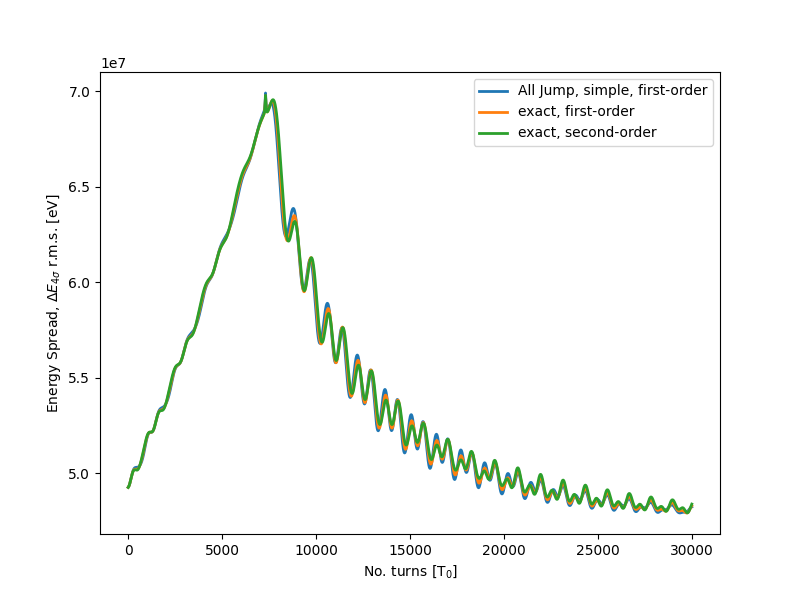
\includegraphics[width=\linewidth]{TEXPaper/img/jump_several_bunch_energy_spread}};
			\end{tikzpicture}
		\end{minipage}
		\begin{minipage}{0.33\linewidth}
			\begin{tikzpicture}
			\node (cone) at (0,0) {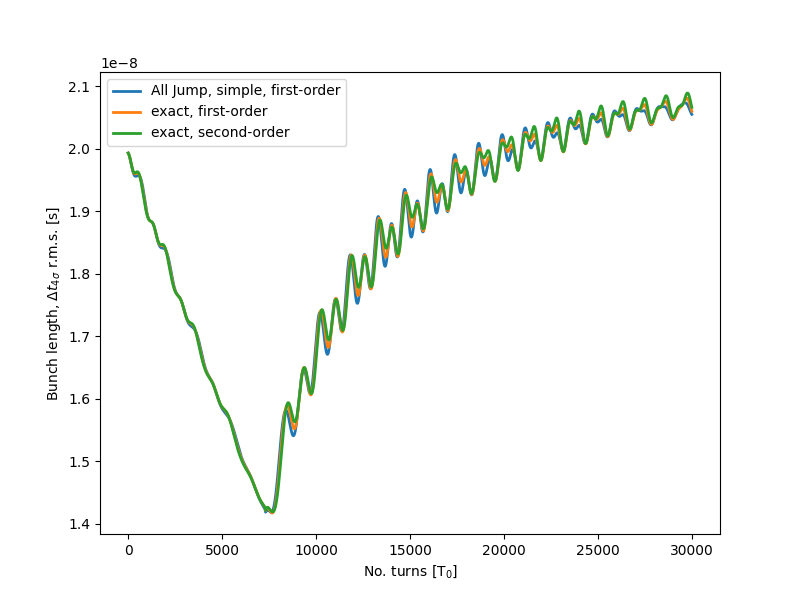
\includegraphics[width=\linewidth]{TEXPaper/img/jump_several_bunch_length_evol}};
			\end{tikzpicture}
		\end{minipage}
		
\par Pure inductive impedances used $Z_{\|}/n=\pm10i$ for various intensity at jump procedure.

		\begin{minipage}{0.33\linewidth}
			\begin{tikzpicture}
			\node (cone) at (0,0) {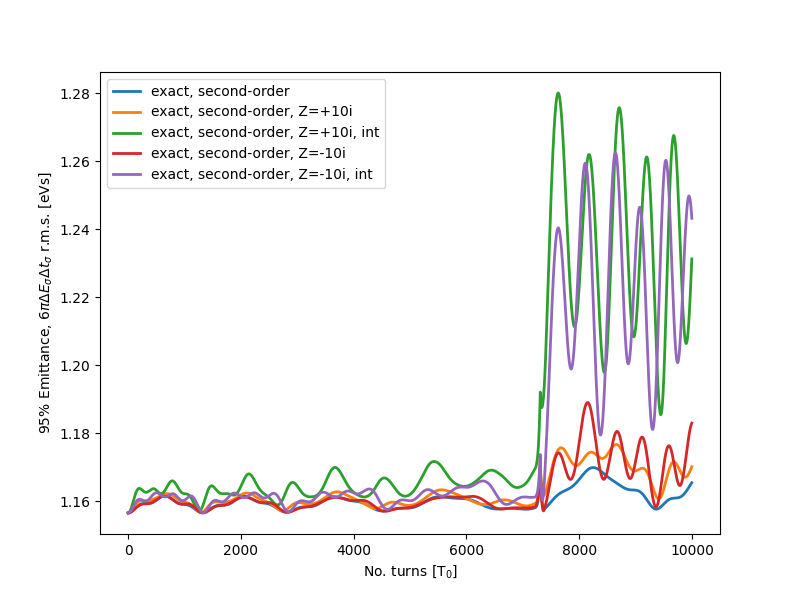
\includegraphics[width=\linewidth]{TEXPaper/img/jump_several_bunch_emittance_sc}};
			\end{tikzpicture}
		\end{minipage}
		\begin{minipage}{0.33\linewidth}
			\begin{tikzpicture}
			\node (cone) at (0,0) {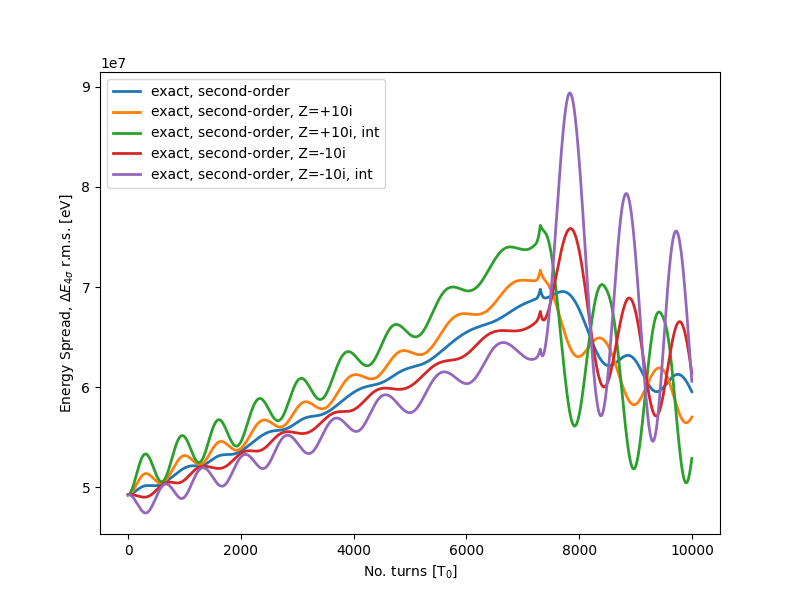
\includegraphics[width=\linewidth]{TEXPaper/img/jump_several_bunch_energy_spread_sc}};
			\end{tikzpicture}
		\end{minipage}
		\begin{minipage}{0.33\linewidth}
			\begin{tikzpicture}
			\node (cone) at (0,0) {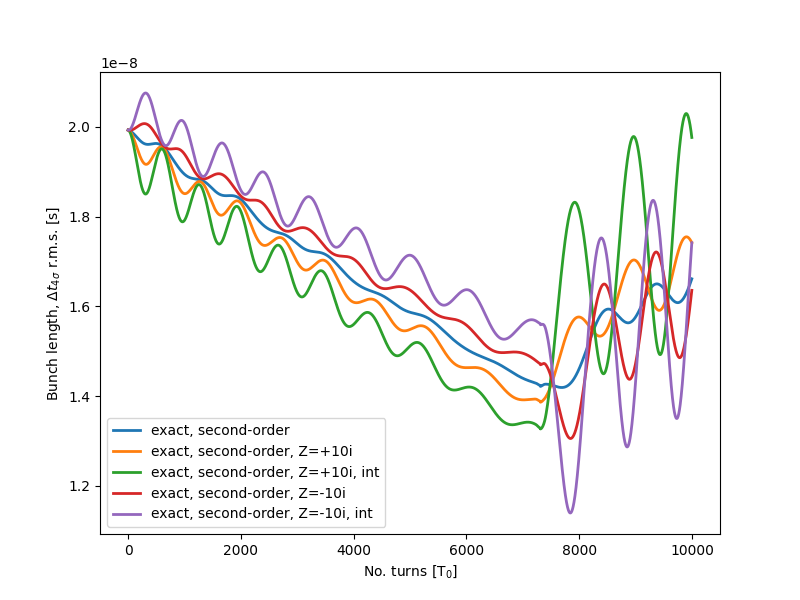
\includegraphics[width=\linewidth]{TEXPaper/img/jump_several_bunch_length_evol_sc}};
			\end{tikzpicture}
		\end{minipage}
\par Small emittance growth compare with non-jump case. In each case of transition crossing, to ensure stability in longitudinal plane, must be considered potentially possible transition energy jump, high orders of momentum compaction factor and impedance induced voltage, especially for intensity beams.
}


\block{Experimental data}{
	
		\begin{minipage}{0.33\linewidth}
		\begin{tikzpicture}
			\node (cone) at (0,0) {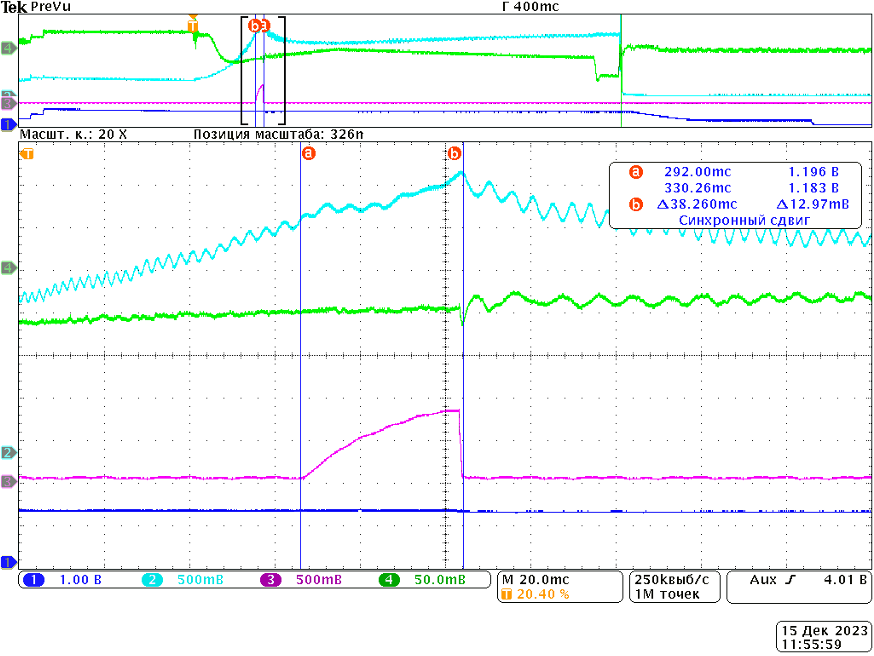
\includegraphics[width=\linewidth]{TEXPaper/img/U-70_jump}};
		\end{tikzpicture}
		\end{minipage}
		\begin{minipage}{0.33\linewidth}
		\begin{tikzpicture}
			\node (cone) at (0,0) {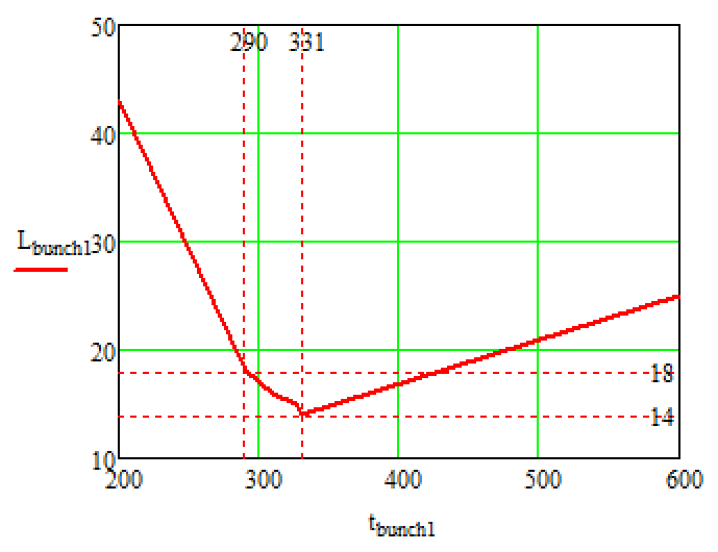
\includegraphics[width=\linewidth]{TEXPaper/img/bunch_lenght}};
		\end{tikzpicture}
		\end{minipage}
		\begin{minipage}{0.33\linewidth}
		\par Experimental data from session at U-70 proton synchrotron carried out at December 2023 in Protvino.
		\end{minipage}
		\par Shown jump-procedure at U-70 Green line -- phase detector, Purple -- gradient in additional quadrupoles, Cyan -- peak detector (inverse proportional to bunch length), Blue -- intensity. And bunch length, which shows  an accordance with modelling of jump procedure.
}			
		
\end{columns}

\begin{columns}
\column{.5}

	\block{CONCLUSION}{
\par The transition energy crossing in harmonic RF, both using the jump method and without it, was considered in a session on the U-70 proton synchrotron. And also by modeling longitudinal dynamics for various orders of slip-factor, impedances and intensities.
It is shown that the rate of acceleration plays a key role in transition crossing. To increase it, the method of raising the transition energy by modulating the dispersion function is used. 
\par The results obtained are of great interest for further study of the transition energy in both harmonic and barrier RF in the NICA collider for accelerating polarized protons.
}

\column{.5}
	\block{REFERENCES}{
	 
	\par [1] S.-Y. Lee, Accelerator Physics (Fourth Edition), DOI:10.1142/11111, ISNB: 978-981-327-468-6, 978-981-327-467-9, World Scientific Publishing Company, 2018.
	\par [2] Pashkov, Proton synchrotron studies.
	\par [3] Ng, K. Y.", Physics of Intensity Dependent Beam Instabilities, U.S. Particle Accelerator School (USPAS 2002), FERMILAB-FN-0713, 2002.
	\par [4] BLonD, https://blond.web.cern.ch/
	\par [5] OptiM, V.A.Lebedev
	}
	
\end{columns}

\end{document}